\graphicspath{{introduction/fig/}}

\chapter{Introduction}
\label{chap:introduction}

The last few years have seen great advances in speech recognition. Much of this progress is due to the resurgence of neural networks; most speech systems now rely on deep neural networks (DNNs) with millions of parameters~\cite{dahl+etal_taslp12,hinton+etal_spm2012}.
However, as the complexity of these models has grown, so has their reliance on labelled training data. Currently, system development requires large corpora of transcribed speech audio data, texts for language modelling, and pronunciation dictionaries.
Despite speech applications becoming available in more languages, it is hard to imagine that resource collection at the required scale would be possible for all 7000 languages spoken in the world today.

I really like apples.

\section{Section heading}

This is some section with two table in it: Table~\ref{tbl:exemplars} and Table~\ref{tbl:abx_speaker}.

\begin{table}[!h]
    \mytable
    \caption{Performance of the unconstrained segmental Bayesian model on TIDigits1 over iterations in which the reference set is refined.}
    \begin{tabularx}{\linewidth}{@{}lCCCCC@{}}
        \toprule
        Metric     & 1 & 2 & 3 & 4 & 5 \\
        \midrule
        WER (\%)                        & $35.4$ & $23.5$ & $21.5$ & $21.2$ & $22.9$ \\
        Average cluster purity (\%)       & $86.5$ & $89.7$ & $89.2$ & $88.5$ & $86.6$ \\
        Word boundary $F$-score (\%)         & $70.6$ & $72.2$ & $71.8$ & $70.9$ & $69.4$ \\
        Clusters covering 90\% of data   & 20             & 13 & 13 & 13 & 13 \\
        \bottomrule
    \end{tabularx}
    \label{tbl:exemplars}
\end{table}


\begin{table}[!h]
    \renewcommand{\arraystretch}{1.1}
    \centering
    \caption{A table with an example of using multiple columns.}
    \begin{tabularx}{0.65\linewidth}{@{}lCCr@{}}
        \toprule
        & \multicolumn{2}{c}{Accuracy (\%)} \\
        \cmidrule(lr){2-3}
        Model    & Intermediate & Output & Bitrate\\
        \midrule
        Baseline & 27.5         & 26.4   & 116 \\
        VQ-VAE   & 26.0         & 22.1   & 190 \\
        CatVAE   & 28.7         & 24.3   & 215 \\
        \bottomrule
    \end{tabularx}
    \label{tbl:abx_speaker}
\end{table}

\newpage

This is a new page, showing what the page headings looks like, and showing how to refer to a figure like Figure~\ref{fig:cae_siamese}.

\begin{figure}[!t]
    \centering
%     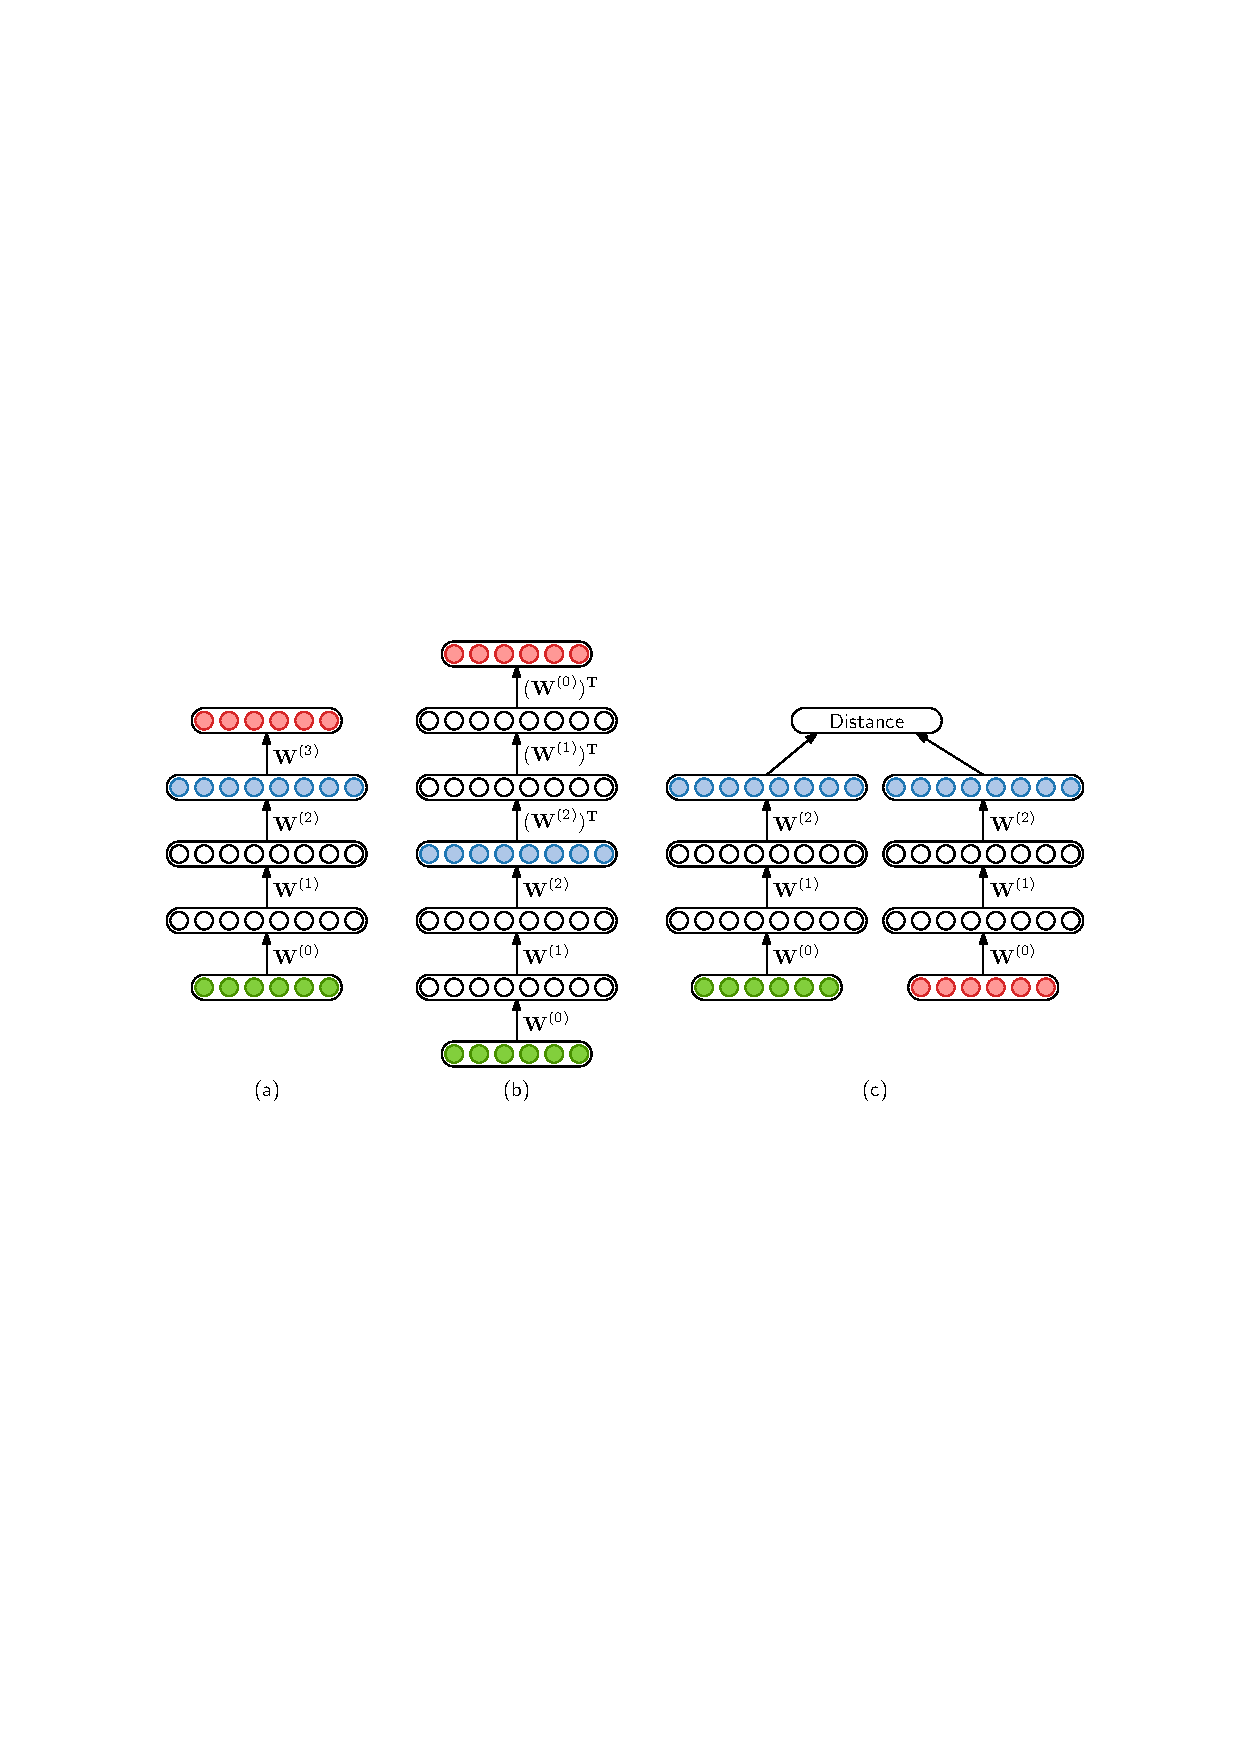
\includegraphics[width=\linewidth]{cae_siamese}
    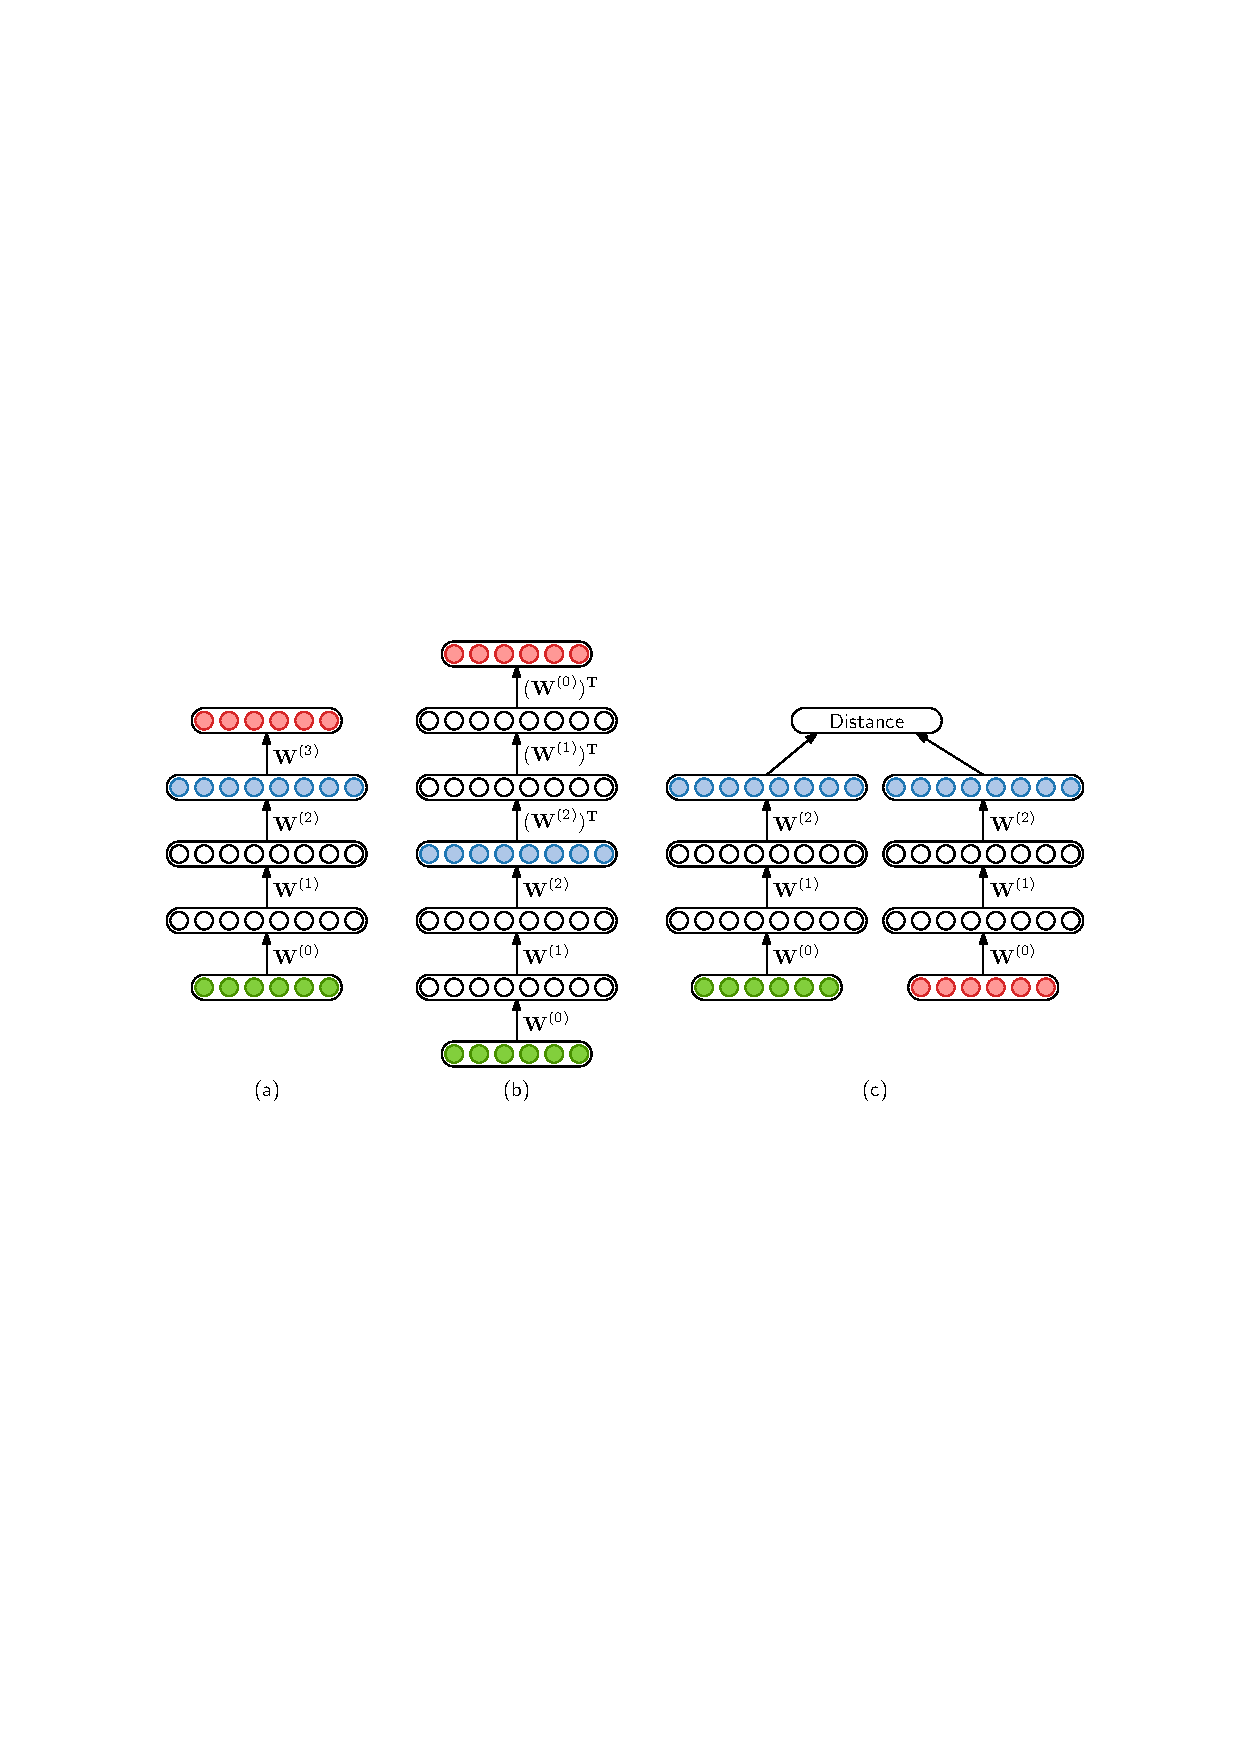
\includegraphics[width=0.918\linewidth]{cae_siamese}
    \caption[I am the short caption that appears in the list of figures, without references.]{
    (a) The cAE as used in this chapter. The encoding layer (blue) is chosen based on performance on a development set.
    (b) The cAE with symmetrical tied weights. The encoding from the middle layer (blue) is always used.
    (c) The siamese DNN. The cosine distance between aligned frames (green and red) is either minimized or maximized depending on whether the frames belong to the same (discovered) word or not.
    A cAE can be seen as a type of DNN~\cite{dahl+etal_taslp12}.
    }
    \label{fig:cae_siamese}
\end{figure}


The following is an example of an equation:
\begin{equation}
P(\vec{z} | \vec{\alpha}) = \int_{\vec{\pi}} P(\vec{z} | \vec{\pi}) \, p(\vec{\pi} | \vec{\alpha}) \, \textrm{d} \vec{\pi}
= \int_{\vec{\pi}} \prod_{k = 1}^K \pi_k^{N_k} \frac{1}{B(\vec{\alpha})} \prod_{k = 1}^K \pi_k^{\alpha_k - 1} \, \textrm{d} \vec{\pi}
\label{eq:example_equation}
\end{equation}
which you can subsequently refer to as~\eqref{eq:example_equation} or Equation~\ref{eq:example_equation}.
But make sure to consistently use the one or the other (and not mix the two ways of referring to equations).






CH1
 Background (1/2 to 1 page) - give context
- background is not what is the problem, but what is the context of the problem. Why does it matter. How many people suffer from lack of clean water for eg or die from car accidents. 

- problem statement (1 paragraph). Most important of entire report. Exactly what you have done. Nothing more or less. sentence or two. 
- objectives "fine-grain" SMART, numbers. If i meet these objectives, i have solved the problem statement in part. 1-5 objectives or sub-objectives or even requirements. Measured against objectives - metrics. 
Summary of work (not contribution for skripsie). what you have achieved. meeting objectives. 
- Scope: What will be done and not be done. Mainly what will not be done. Did not take into account organic material or eg did not consider mobility. Did think about other things - still important (e.g. future work). write it in such a way that it is positive  / what u did do. did not consider cost size market manufacturability etc. 
- Structure of Report (Not exactly the same as the Table of Contents): Roadmap, in chapter 2 I did the following etc

ECSA chapter 1: I took a vaguely defined problem (prob statement), understood what i must do to solve (objectives), and then solved it (summary of work).
Then, 


CH2

LIT-review + background concept (4th year)
- Previous Work done in this field or goal
which other solutions exist that try to do the same thing. 
1. related work - summary of other solutions (academia or industry). 1.  What their objectives were (vaguely similar). What method did they employ (how go abt or measuring the thing or validating their solution). what were their results. What were there shortcomings - what did they not do that answers ur prob statement. E.g. wont work in africa (remaining challenges).

2. What information did u draw from or acquire to solve problem. What did I learn not from EE engineering. Additional to undergrad. 

e.g. water quality: UV spectrum, optical sensing, color spectrum moving signals. Capture additional technologies and information to do design. Anything beyond scope of EE, lecturer might not know. I needed to know this before addressing problem. 


eg i have these 3 options at my disposal or many. 

CH3
System design - functional blocks of whole system. e.g. water quality: sensor, microcontroller, communication, power supply. or software flow model. or UAV model. ch3 must list options at my disposal.  for each functional block in system must say why u chose it. eg three sesnsors for optical sensors, but I chose UV sensor because of this. eg 100 feature extractors i chose 1 or 10. dont calculate minute details eg resistor values. power or data flow. 
high level system design. each block has its own section e.g. text or copy paste block. no mention of sub blocks. 

section 2: metrics. Does it respond to xyz. is it proportional. false positives. what do we intend to measure and how do we intend to do so (oscilloscope or printout). Must tie up to objectives set. can start chapter 3 with a list of requirements - metrics must prove requirements (repeat objectives).

Software eg: I chose monga database. had option of x databases and chose monga for these reasons. 

If skripsie more research:
may call it method, or experimental setup. 

Ch4
detailed design. For each functional block how did u design the minute details. Mirror (copy paste) the same block. how u filled block eg once again i chose option 1. i chose this resistor value. 

Software eg: how did i setup the monga database to meet requirements. all fields of database. 
quick results, resistor got hot changed it. intermediate results. 


Results
NO DESIGN. NO justification. no requirements or objectives. just dumb results - dont link back. each fig must have descriptive caption. one sentence. 

1. what.In figure 1a,  we are looking at the response of doing this when doing this. What are they looking at. we looking at measurement of temperature when sun shines. 
2. second sentence. what is it that u r showing the reader. when we look at this we can see temp peak is in middle of day. what r we observing or taking from image. 
3. now that ive observed that strange or expected behaviour what does it tell u. peak in middle of day, sensor is working. short burst of current in middle of day, will have to fix it or fix in next iteration. 

do for each table. and this body of results must correspond to what we said we will measure; to meet requirements or objectives. 

Conclusion. 
quick repeat for reader, this is what we tried to do, this is what i gave in report, 
list objectives. 
1. obj 1, i used this metric, reference section or image, and i got the following results.
2. another obj and how we method

finally, so what. what can we say. mirrors chapter 1 background and problem statement. all past tense. what are we gonna tell our granny at the braai (ai prediction). this means that people in rural areas (water quality monitor) can use the sensor to do the following. NB, but more work needs (limitation or caution) to be done in the middle of the day to fix issue. 
future work. recommendations. 

CH3 -> CH x-2
Conceptual -> Detailed Design

CH x-1
Results + Evaluation (NB!)

CH x
Conclusion, future work and limitations



\section{Background}
\begin{itemize}
    \item \textbf{Problem Statement:}
    \begin{itemize}
        \item Most current UAV navigation systems are purely GPS-based, which is susceptible to new GPS-denial technology. Additionally, existing solutions mainly involve emission technology (e.g., LIDAR) which can be detected by oppositions.
    \end{itemize}
    \item \textbf{Motivation:}
    \begin{itemize}
        \item There is a need for a navigation redundancy system that avoids detection in GPS-denied environments.
    \end{itemize}
    \item \textbf{Literature Review:}
    \begin{itemize}
        \item UAV navigation and GPS Dependency.
        \item Alternative Navigation Methods.
        \item Feature Detection and Matching.
        \item Homographic estimation. 
        \item Stereo Vision. 
        \item Computational Requirements. 
    \end{itemize}
\end{itemize}

\section{Aims and Objectives}
\begin{itemize}
    \item \textbf{Aim:}
    \begin{itemize}
        \item Develop a robust and accurate image-based GPS location estimator for UAV navigation post-GPS signal loss. 
    \end{itemize}
    \item \textbf{Objectives:}
    \begin{itemize}
        \item Design, develop and test algorithms for efficient, robust and accurate feature extraction and feature matching. This will be used during flight and matched with known GPS locations and heading. The system requires at least 500 matches to be sufficiently confident. 
        \item Upon GPS-signal loss, use the above to compare current and prior images to estimate the translation and rotation of the UAV, thereby inferring the current GPS location and heading of the UAV. The system shall have a normalize x, y error under 100m and a heading error under 10 degrees.
        \item Improve the above method by utilizing stereo vision for depth awareness and increased accuracy. 
        \item Implement the system on a single-board computer (SBC) for real-time operation. The system shall have a processing time of under 10s per frame in the forward flight, and under 3s per frame in the backward flight.
    \end{itemize}
\end{itemize}

\section{Scope}
\begin{itemize}
    \item \textbf{Assumptions and Restrictions:}
    \begin{itemize}
        \item Real-life data from a UAV test-flight will be used. This data shall be from a perfectly downwards view, sufficiently detailed and distortion-free (e.g., warping, blurring, clouds, etc.).
        \item No roll and pitch changes will occur during the flight.
        \item The UAV will be flying at a constant altitude.
        \item The system output is an estimated GPS location and heading estimate, not a control system.
    \end{itemize}
\end{itemize}

\section{Methods and Approach}
\begin{itemize}
    \item \textbf{Data Collection:}
    \begin{itemize}
        \item Capture sequential images from UAV flights at different altitudes.
        \item The UAV should follow a predefined path with known GPS coordinates, heading, camera parameters, and altitude. Thereafter, the UAV should fly very close to the same path backward.
    \end{itemize}
    \item \textbf{Design and Development:}
    \begin{itemize}
        \item Research and test the accuracy and count of features in 5-10 different feature extraction methods. 
        \item Research and test the accuracy and count of matches in 5-10 different feature matching methods.
        \item Implement and evaluate different homographic estimation methods. 
        \item Implement and evaluate stereo vision methods.
        \item Implement and evaluate the system on a SBC.
    \end{itemize}
    \item \textbf{Analysis:}
    \begin{itemize}
        \item Use sequential image analysis to estimate new coordinates.
        \item Implement and evaluate pathfinding algorithms to calculate a path backward using past captured features.
    \end{itemize}
\end{itemize}

\section{Structure}

\begin{itemize}
    \item \textbf{Chapter 2: Literature Review}
    \begin{itemize}
        \item Discusses the current state of UAV navigation and GPS dependency, alternative navigation methods, feature detection and matching, homographic estimation, stereo vision, and computational requirements.
    \end{itemize}
    \item \textbf{Chapter 3: Methodology}
    \begin{itemize}
        \item Describes the data collection, design and development, and analysis methods used in the project.
    \end{itemize}
    \item \textbf{Chapter 4: Results}
    \begin{itemize}
        \item Presents the results of the project, including the accuracy and efficiency of the developed system.
    \end{itemize}
    \item \textbf{Chapter 5: Discussion}
    \begin{itemize}
        \item Discusses the implications of the results and the potential impact of the project.
    \end{itemize}
    \item \textbf{Chapter 6: Conclusion}
    \begin{itemize}
        \item Summarizes the project and its outcomes.
    \end{itemize}
\end{itemize}



\section{Potential Impact}
\begin{itemize}
    \item \textbf{Societal Impact:}
    \begin{itemize}
        \item Enhance the reliability of UAV operations in civilian applications such as disaster response and border patrol.
    \end{itemize}
    \item \textbf{Knowledge Impact:}
    \begin{itemize}
        \item Contribute to advancements in UAV navigation technology and computer vision applications.
    \end{itemize}
    \item \textbf{Economic Impact:}
    \begin{itemize}
        \item Increase the practicality and usage of UAV systems in military and civilian contexts, potentially enhancing border control, enhancing international electronic engineering collaboration.
    \end{itemize}
    \item \textbf{Safety Impact:}
    \begin{itemize}
        \item Increase the ability for national surveillance missions to secure critical knowledge in a military context.
    \end{itemize}
\end{itemize}

\section{Conclusion}
\begin{itemize}
    \item The project aims to improve UAV navigation accuracy and reliability in GPS-denied environments through camera-based image matching. This may have profound impacts in a South African military context as well as broader impacts on civil safety and economic well-being.
\end{itemize}

\section*{References}
\begin{enumerate}
    \item Sathyamoorthy, D., et al. (2020). Evaluation of the Vulnerabilities of Unmanned Aerial Vehicles (UAVs) to Global Positioning System (GPS) Jamming and Spoofing. \textit{Defense Science \& Technology Journal}, 33, 334-343.
    \item Rusnák, M. \& Vásárhelyi, J. (2023). A review of using visual odometry methods in autonomous UAV navigation in GPS-denied environment. \textit{Acta Universitatis Sapientiae Electrical and Mechanical Engineering}, 15, 14-32. \url{https://doi.org/10.2478/auseme-2023-0002}
    \item Karab, E., Prasad, S., \& Shahato, M. (2017). Image Matching Using SIFT, SURF, BRIEF and ORB: Performance Comparison for Distorted Images. \textit{Acta Polytechnica Hungarica}, 14(6), 183-206.
    \item Luglio-Miguel, F., Iores, G., \& Salazar, S. \& Lozanc, R. (2014). Dubins path generation for a fixed-wing UAV. \textit{Proceedings of the International Conference on Unmanned Aircraft Systems (ICUAS)}, 339-345.
\end{enumerate}
